% $HeadURL$

\subsection{Glyph: \glyph{Genetic Entity}}
\label{sec:genetic}

The \emph{genetic entity} construct in SBGN is meant to represent a fragment of a macromolecule carrying genetic information.  A common use for this construct is to represent a gene or transcript.  The label of this EPN and its \emph{units of information} are often important for making the purpose clear to the reader of a diagram.

\begin{glyphDescription}

\glyphSboTerm SBO:0000354 ! genetic entity

\glyphContainer A \glyph{genetic entity} is represented by a rectangular container whose bottom half has rounded corners, as shown in \fig{genetic}.

\glyphLabel The identity of a particular \glyph{genetic entity} is established by a label placed in an unordered box containing a string of characters.  The characters may be distributed on several lines to improve readability, although this is not mandatory.  The label box must be attached to the center of the container.  The label may spill outside of the container.

\glyphAux A \glyph{genetic entity} can carry state variables (\sect{stateVariable}) that add information about its precise state.  The state of a genetic entity is therefore defined as the vector of all its state variables.  A state variable is represented by an ellipsoid container, with the long axis of the ellipsoid placed on the border of the \glyph{genetic entity}'s container as illustrated in \fig{genetic}.  The label of the state variable (type of characteristic, nucleotide number) can be optionally written either within the \glyph{genetic entity} container, or next to the border of the state variable container, or within the variable's container itself.

A \glyph{genetic information} can also carry one or several \glyph{units of information} (\sect{unitInfo}).  These can characterise a \glyph{genetic entity}'s domain, such as a binding site, or an exon.  Particular \glyph{units of information} carry the material type (\sect{material-types-cv}) and the conceptual type (\sect{conceptual-types-cv}) of the of the genetic entity.  The center of the bounding box of a \glyph{unit of information} is located on the midline of the border of the \glyph{genetic entity}.

A \glyph{genetic entity} may also carry a \glyph{clone marker}
(\sect{cloneMarker}).

\end{glyphDescription}


\begin{figure}[H]
  \centering
  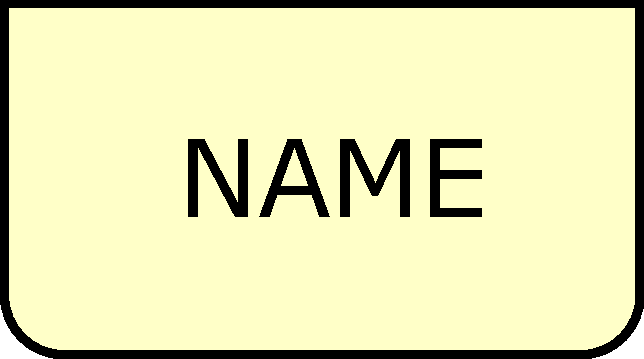
\includegraphics[scale = 0.3]{images/genetic}
  \caption{The \PD glyph for \glyph{genetic entity}.}
  \label{fig:genetic}
\end{figure}




% The following is for [X]Emacs users.  Please leave in place.
% Local Variables:
% TeX-master: "../sbgn_PD-level1"
% End:
